\documentclass[11pt,a4paper]{article}

\usepackage[utf8]{inputenc}
\usepackage[T1]{fontenc}
\usepackage{lmodern}
\usepackage[margin=1in]{geometry}
\usepackage{setspace}
\usepackage{amsmath,amssymb,amsfonts,amsthm,mathtools}
\usepackage{array}
\usepackage{booktabs}
\usepackage{graphicx}
\usepackage[hidelinks]{hyperref}
\usepackage{enumitem}
\usepackage{tabularx}
\usepackage{float}
\usepackage[hypcap=false]{caption}

\setstretch{1.1}
\emergencystretch=2em

\newtheorem{theorem}{Theorem}[section]
\newtheorem{proposition}[theorem]{Proposition}
\newtheorem{corollary}[theorem]{Corollary}
\theoremstyle{definition}
\newtheorem{definition}[theorem]{Definition}
\theoremstyle{remark}
\newtheorem{remark}[theorem]{Remark}

\newcommand{\dec}{\Lambda_{\mathrm{dec}}}
\newcommand{\diag}{\mathrm{diag}}
\newcommand{\off}{\mathrm{off}}
\newcommand{\bures}{g_B}
\newcolumntype{Y}{>{\raggedright\arraybackslash}X}
\graphicspath{{figures/}}

\title{Information Geometry of Classical Carriers and\\ Non-Classical Payloads in Biological Information Processing}
\author{Ian Todd\thanks{ORCID: 0009-0002-6994-0917; Email: itod2305@uni.sydney.edu.au}\\
Sydney Medical School\\
University of Sydney\\
Sydney, Australia}
\date{}

\begin{document}

\maketitle

\begin{abstract}
Decoherence maps a $d$-level quantum system from a $(d^2-1)$-dimensional Bures manifold onto a $(d-1)$-dimensional Fisher--Rao simplex, annihilating the coherence directions. This dimensional collapse yields a continuous non-classicality index $\chi$ from Bures principal angles, quantifying how much coherence-sector structure remains geometrically accessible at any operating point. We apply that geometry to biological systems. Photosynthetic complexes provide the proof of principle, operating near the quantum-classical boundary with small but nonzero $\chi$. A minimal ion-channel selectivity-filter model and a coarse protein-microdomain model occupy the same near-boundary band, while neural carrier proxies sit deep in the classical regime. These anchors motivate a \emph{carrier-payload architecture}: deep-classical macroscopic carriers coordinate an extensive near-boundary molecular substrate. The total non-classical payload grows linearly with the number of entrained modules whenever a nonzero fraction sits near the boundary and redundancy is bounded. This architecture implies a concrete hybrid simulation protocol: carrier dynamics are simulated classically, while near-boundary payload modules are treated as small open quantum systems via Lindblad equations. Under the assumption that inter-module quantum correlations remain negligible and coupling is classical, the protocol scales linearly in module count, and $\chi$ serves as a screening heuristic for which modules need quantum treatment. More speculatively, the carrier-payload architecture suggests an engineering direction for computing systems in which a classical oscillatory backbone synchronizes many slightly non-classical processing elements, replacing qubit isolation with coordinated payload breadth.
\end{abstract}

\noindent\textbf{Keywords:} decoherence; information geometry; quantum-classical boundary; biological organization; hybrid simulation; carrier-payload architecture

\bigskip
\noindent\textbf{Highlights}
\begin{itemize}[nosep,leftmargin=*]
\item Decoherence is formalized as dimensional collapse from $d^2{-}1$ to $d{-}1$ dimensions, yielding a continuous non-classicality index $\chi$.
\item Photosynthetic, ion-channel, and protein-microdomain anchors inhabit a near-boundary band; neural carriers are substantially more classical.
\item The non-classical payload is extensive in entrained module count, giving a carrier-payload architecture for multi-scale biological systems.
\item A hybrid simulation protocol follows directly: classical carrier dynamics plus small Lindblad equations for near-boundary payload modules, scaling linearly when inter-module correlations are negligible.
\item The same architecture suggests an engineering hypothesis in which classical oscillatory coordination replaces qubit isolation.
\end{itemize}

\section{Introduction}
\label{sec:intro}

Biological systems operate productively at the quantum-classical boundary. Igamberdiev and colleagues have argued for decades that this is not accidental: living systems exploit the interplay between quantum-mechanical constraints and classical information processing to achieve computational and organizational capacities that neither regime alone could sustain \cite{igamberdiev1993,igamberdiev2021qcborder}. Photosynthetic complexes show environment-assisted quantum transport at physiological temperatures \cite{engel2007evidence,mohseni2008environment,plenio2008dephasing,cao2020quantum}. Ion channels, enzyme active sites, and protein-folding intermediates operate at energy scales where the boundary between quantum coherence and thermal decoherence is not remote but immediate.

What has been missing is a \emph{geometric} framework for saying where a given biological system sits on that boundary and what the boundary position costs or enables. The present paper supplies such a framework. Decoherence is the standard physical route from quantum to classical descriptions \cite{zeh1970interpretation,zurek2003decoherence,schlosshauer2005decoherence}. A $d$-level quantum system occupies a $(d^2-1)$-dimensional state manifold under the Bures metric \cite{bures1969extension,braunstein1994statistical,petz1996monotone}. Complete dephasing collapses this manifold onto the $(d-1)$-dimensional classical probability simplex under the Fisher--Rao metric \cite{rao1945information,amari1985differential}. The collapse destroys $d^2-d$ coherence directions. We define a continuous non-classicality index $\chi\in[0,1]$ from the Bures principal angles between classical and coherence tangent subspaces. This index places any system on a geometric spectrum from fully classical ($\chi=0$) to maximally coherent ($\chi=1$), without forcing a binary classification.

Applied to biology, $\chi$ reveals a consistent pattern. Validated photosynthetic Hamiltonians (FMO, PE545) produce operating points with small but nonzero $\chi$ --- the near-boundary regime where function is already known to reside. A minimal ion-channel selectivity-filter model and a coarse protein-microdomain model occupy the same band. Neural oscillations, by contrast, sit deep in the classical regime ($\chi_{\mathrm{carrier}} \ll \chi_{\mathrm{payload}}$). This separation motivates a \emph{carrier-payload architecture}: deep-classical macroscopic processes coordinate an extensive near-boundary molecular substrate.

Two practical consequences follow. First, the architecture implies a \emph{hybrid simulation protocol} for multi-scale biological systems. Carrier dynamics are simulated classically; near-boundary payload modules are simulated as small open quantum systems (Lindblad equations of dimension $d\sim 4$--$10$). When inter-module quantum correlations are negligible and coupling is classical, the protocol scales linearly in entrained module count rather than exponentially in Hilbert-space dimension, and $\chi$ serves as a screening heuristic for which modules merit quantum treatment. Second, the same architecture suggests a \emph{speculative engineering direction}: instead of isolating fragile qubits, one could synchronize many slightly non-classical processing elements via a classical oscillatory backbone, replacing qubit fidelity with coordinated payload breadth.

The paper develops these ideas in four steps. Section~\ref{sec:geometry} states the core geometric facts and defines $\chi$. Section~\ref{sec:architecture} builds the carrier-payload formalism. Section~\ref{sec:anchors} uses photosynthesis as proof of principle and then prioritizes ion channels as the leading neural payload candidate, with protein microdomains as a secondary extension. Section~\ref{sec:consequences} develops the multi-scale coordination model, states the simulation protocol, and derives empirical predictions. The central outcome is a change of analytical perspective: the question ``is this system quantum or classical?'' is replaced by ``what is its $\chi$, how is the near-boundary payload distributed, and what simulation or design architecture follows?''

The burden of proof is stratified. The geometric statements in Sections~\ref{sec:geometry} and \ref{sec:architecture} are theorem-level claims. The biological anchors are model-based computations from validated or illustrative Hamiltonians. The simulation protocol and computing-architecture implications are methodological consequences of the framework. The paper does not claim that the non-classical payload is already known to be functionally decisive for cognition; it establishes that the payload is nonzero, geometrically structured, extensive, and empirically testable.

\medskip
\noindent\fbox{\parbox{\dimexpr\linewidth-2\fboxsep-2\fboxrule}{%
\textbf{On ``dimensionality.''} Throughout this paper we use \emph{dimensionality} in the \textbf{ML/complex-systems sense}: the effective/intrinsic degrees of freedom of accessible dynamics (e.g., participation ratio or effective rank of covariance/response spectra, or measure of the coherently accessible region)---\textbf{not} geometric embedding dimension. Measurement is dimensional collapse.}}
\medskip

\section{Geometry of the Quantum-Classical Boundary}
\label{sec:geometry}

\subsection{Dimensional collapse under dephasing}

Let $\mathcal{M}_Q$ denote the manifold of $d\times d$ density matrices. For a full-rank system, $\dim \mathcal{M}_Q = d^2-1$: there are $d-1$ independent populations and $d^2-d$ off-diagonal coherence directions. Fix a pointer basis $\{\lvert k\rangle\}_{k=1}^d$ and let
\begin{equation}
\label{eq:dephasing}
\dec(\rho)=\sum_{k=1}^d \lvert k\rangle\langle k\rvert\,\rho\,\lvert k\rangle\langle k\rvert
\end{equation}
be the complete dephasing channel.

\begin{theorem}[Dimensional collapse]
\label{thm:collapse}
Under complete dephasing, the $(d^2-1)$-dimensional quantum manifold collapses onto the $(d-1)$-dimensional classical probability simplex:
\begin{equation}
\label{eq:collapse}
d^2-1 \longrightarrow d-1.
\end{equation}
Equivalently, the $d^2-d$ off-diagonal coherence directions are annihilated, and the Bures metric on the image of $\dec$ restricts to the Fisher--Rao metric.
\end{theorem}

\begin{proof}
The image of $\dec$ is the set of diagonal density matrices, which is the classical simplex $\Delta_{d-1}$. Any derivative in an off-diagonal direction vanishes after applying $\dec$, so those directions drop out of the quantum Fisher information matrix. For a diagonal state $\rho=\mathrm{diag}(p_1,\ldots,p_d)$ and a tangent vector $\delta\rho=\mathrm{diag}(\delta p_1,\ldots,\delta p_d)$ with $\sum_k\delta p_k=0$, the Bures/SLD metric reduces to $\sum_k (\delta p_k)^2/p_k$, i.e.\ the Fisher--Rao metric on the simplex \cite{braunstein1994statistical,petz1996monotone,rao1945information}. Hence only $d-1$ distinguishable directions remain.
\end{proof}

\subsection{Principal angles and non-classicality}

At a diagonal state, diagonal and off-diagonal tangent directions are orthogonal under the Bures metric. Away from the simplex they need not be orthogonal; the failure of orthogonality is exactly what it means for classical and quantum directions to remain mixed.

\begin{definition}[Non-classicality index]
\label{def:chi}
Let $\theta_1,\ldots,\theta_{d-1}$ be the Bures principal angles between the diagonal and off-diagonal tangent subspaces at a full-rank state $\rho$. Define
\begin{equation}
\label{eq:chi}
\chi(\rho)=\frac{1}{d-1}\sum_{a=1}^{d-1}\cos^2\theta_a.
\end{equation}
\end{definition}

By construction, $\chi(\rho)\in[0,1]$. Diagonal states have $\theta_a=\pi/2$ for all $a$, hence $\chi=0$. Any state with geometric mixing between classical and coherence directions has $\chi>0$. The index is deliberately modest: it is not an entanglement measure, not a coherence monotone, and not a claim that a system is ``quantum'' in any maximal sense. It is a scalar summary of how much of the coherence sector remains geometrically accessible. In the biological applications below, $\chi$ is evaluated on the full-rank regularized readout state produced by the corresponding Lindblad model at the stated operating point.

\begin{remark}
\label{rem:highd}
Large dimensionality alone does not imply non-classicality. A very large classical system can still satisfy $\chi=0$. The claim developed below is therefore extensive rather than ontological: if a system contains many modules with small but nonzero local $\chi_i$, the total payload can scale with system size.
\end{remark}

\section{Carrier-Payload Architecture}
\label{sec:architecture}

\subsection{Local payload load}

To move from single systems to biological assemblies, we distinguish the \emph{carrier} from the \emph{payload}. The carrier is the large-scale coordinating process. The payload is the set of local modules whose internal state spaces are being coordinated.

\begin{definition}[Local non-classical load]
\label{def:local-load}
For module $i$ with local dimension $d_i$ and non-classicality $\chi_i$, define
\begin{equation}
\label{eq:local-load}
L_i=\chi_i(d_i^2-d_i).
\end{equation}
\end{definition}

The term $d_i^2-d_i$ is the size of the coherence sector that decoherence would destroy under full projection. Multiplying by $\chi_i$ gives a geometry-weighted effective load.

\subsection{Redundancy-adjusted effective payload}

Biological modules are not independent. If many modules are strongly redundant, naive linear addition overcounts the accessible payload. We therefore carry an explicit redundancy penalty.

\begin{definition}[Effective payload]
\label{def:payload}
Let $E$ be a set of entrained modules and let $\varrho_E\ge 1$ be a redundancy factor. Define
\begin{equation}
\label{eq:payload}
\mathcal{L}_{\mathrm{eff}}(E)=\frac{1}{\varrho_E}\sum_{i\in E}L_i
\end{equation}
and the effective coordinated-dimension score
\begin{equation}
\label{eq:dcoord}
D_{\mathrm{coord}}(E)=\sum_{i\in E}(d_i-1)+\mathcal{L}_{\mathrm{eff}}(E).
\end{equation}
\end{definition}

The first term counts the surviving classical simplex dimensions. The second term counts the residual geometrically accessible coherence sector after redundancy compression. The sum is an effective geometry score for accessible state-space richness, not a literal manifold-dimension identity.

\subsection{Extensive payload under nonzero module density}

\begin{proposition}[Extensive non-classical payload]
\label{prop:extensive}
Let $E_N$ be an entrained set of $N$ modules. Assume:
\begin{enumerate}[label=\emph{(\roman*)}]
\item there exist constants $L_\star>0$ and $p>0$ such that at least a fraction $p$ of modules in $E_N$ satisfy $L_i\ge L_\star$;
\item the redundancy factor is uniformly bounded, $\varrho_{E_N}\le \varrho_\star$.
\end{enumerate}
Then
\begin{equation}
\label{eq:extensive-bound}
\mathcal{L}_{\mathrm{eff}}(E_N)\ge \frac{pL_\star}{\varrho_\star}N,
\end{equation}
and hence the non-classical payload is extensive in $N$.
\end{proposition}

\begin{proof}
At least $pN$ modules contribute load at least $L_\star$, so $\sum_{i\in E_N}L_i\ge pNL_\star$. Dividing by the bounded redundancy factor gives the stated bound.
\end{proof}

\subsection{Low-frequency advantage as a coordination statement}

\begin{corollary}[Low-frequency carrier advantage]
\label{cor:lowf}
Let $f_1<f_2$ be two carrier frequencies with entrained sets $E(f_1)$ and $E(f_2)$. Suppose:
\begin{enumerate}[label=\emph{(\roman*)}]
\item $\lvert E(f_1)\rvert \ge \lvert E(f_2)\rvert$;
\item the local payload statistics and redundancy bounds remain comparable across the two sets.
\end{enumerate}
Then
\begin{equation}
\label{eq:lowf}
D_{\mathrm{coord}}(E(f_1))\ge D_{\mathrm{coord}}(E(f_2)).
\end{equation}
\end{corollary}

\begin{proof}
Apply Proposition~\ref{prop:extensive} with comparable module statistics and bounded redundancy. The coordinated dimensionality grows with the number of entrained payload modules, not with carrier frequency itself.
\end{proof}

Low frequency is not valuable because it is intrinsically high-dimensional. It is valuable because it can coordinate a larger ensemble while staying close to a classical carrier limit.

\section{Biological Anchors}
\label{sec:anchors}

\subsection{Photosynthesis as proof of principle}

Photosynthetic exciton transport is the cleanest biological proof of principle because the quantum-to-classical tradeoff is already functionally established \cite{engel2007evidence,mohseni2008environment,plenio2008dephasing,rebentrost2009environment,cao2020quantum}. In calculations based on the validated Hamiltonians of Adolphs--Renger and Novoderezhkin \cite{adolphs2006proteins,novoderezhkin2010excitation}, the transport optimum occurs in a near-classical regime rather than at maximal coherence. Averaging over the two standard initial-site choices, FMO gives $\gamma_{\mathrm{opt}}/J_{\max}\approx 1.53$ with $\theta_{\min}^{\mathrm{opt}}\approx 87.96^\circ$, while PE545 gives $\gamma_{\mathrm{opt}}/J_{\max}\approx 7.87$ with $\theta_{\min}^{\mathrm{opt}}\approx 89.02^\circ$. At the biological operating point, the scans give $\theta_{\min}^{\mathrm{bio}}\approx 87.67^\circ$ (FMO) and $89.02^\circ$ (PE545). In local-load units $L=\chi(d^2-d)$, those same biological points correspond to $L_{\mathrm{FMO}}^{\mathrm{bio}}\approx 2.28\times10^{-2}$ and $L_{\mathrm{PE545}}^{\mathrm{bio}}\approx 4.93\times10^{-3}$. This is exactly the regime the present framework is built to describe: biologically relevant function with $\chi>0$ but principal angles already close to $\pi/2$.

The role of photosynthesis in this paper is strategic: it shows that the near-boundary regime is not empty rhetoric. Table~\ref{tab:anchors} and Figure~\ref{fig:anchor-map} summarize the anchor set and show the carrier-payload separation: molecular payload anchors cluster in the same near-boundary band, while neural carrier proxies sit farther right and closer to the classical limit. The ion-channel local load $L_{\mathrm{ion}}\approx 3.31\times10^{-3}$ is of the same order as PE545, so the neural payload anchor is not being placed in a wholly alien regime.

\begin{table}[H]
\centering
\small
\begin{tabularx}{\linewidth}{@{}>{\raggedright\arraybackslash}p{1.3cm}>{\raggedright\arraybackslash}p{1.25cm}>{\raggedright\arraybackslash}p{0.95cm}c c c >{\raggedright\arraybackslash}X@{}}
\toprule
System & Role & Type & $\gamma_{\mathrm{bio}}/J_{\max}$ & $\theta_{\min}^{\mathrm{bio}}$ & $\chi^{\mathrm{bio}}$ & Use in draft \\
\midrule
FMO & Proof point & Direct & 1.14 & $87.67^\circ$ & $5.42\times 10^{-4}$ & Functional near-boundary photosynthesis anchor. \\
PE545 & Proof point & Direct & 7.88 & $89.02^\circ$ & $8.80\times 10^{-5}$ & Independent photosynthetic confirmation of the same band. \\
Ion channel & Neural payload & Direct & 6.67 & $88.55^\circ$ & $2.76\times 10^{-4}$ & Molecular anchor for the primary neural payload route. \\
Prot.\ microd. & Payload ext. & Direct & 7.69 & $88.21^\circ$ & $3.66\times 10^{-4}$ & Secondary payload anchor outside ion conduction. \\
Synth.\ carrier & Carrier & Proxy & 50 & $89.78^\circ$ & $3.72\times 10^{-6}$ & Synthetic gamma-band carrier proxy, already near classical. \\
P-D carrier & Carrier & Proxy & 50 & $89.37^\circ$ & $2.83\times 10^{-5}$ & Potjans--Diesmann cortical-column proxy \cite{potjans2014cell}, still more classical than the payload band. \\
\bottomrule
\end{tabularx}
\caption{Anchor systems. All rows are computed directly. The photosynthetic models use validated Hamiltonians. The neural rows report carrier proxies at $\gamma/J_{\max}=50$ rather than the true biological limit $\gamma_{\mathrm{bio}}/J_{\max}\gg 1$; the latter only pushes the carriers further toward the classical limit.}
\label{tab:anchors}
\end{table}

\begin{figure}[H]
\centering
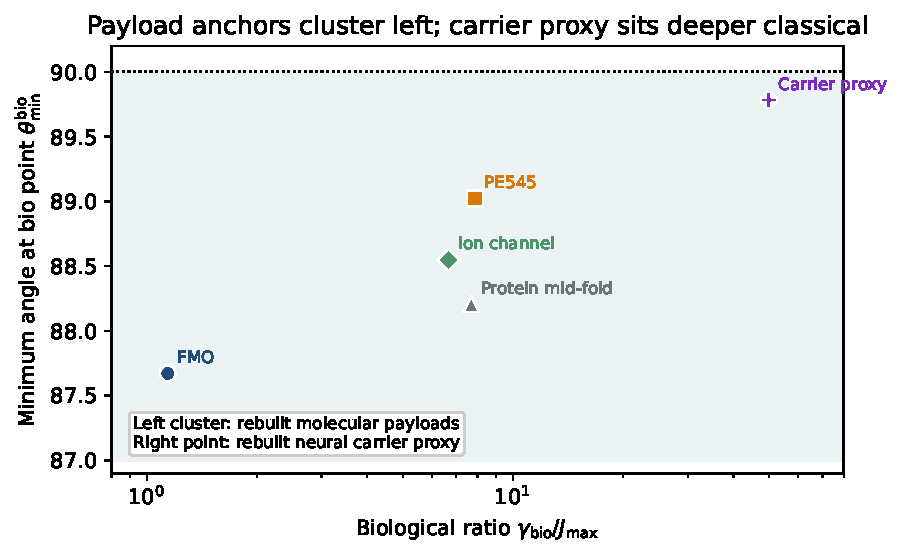
\includegraphics[width=0.72\linewidth]{biological_anchor_map.pdf}
\caption{Biological operating points. The molecular payload anchors --- FMO, PE545, the ion-channel point, and the protein mid-fold point --- cluster in a near-boundary band ($\theta_{\min}^{\mathrm{bio}}$ between roughly $87.7^\circ$ and $89.0^\circ$). Two neural carrier proxies sit farther right at $\gamma/J_{\max}=50$ and closer to the classical limit. This visual separation is the paper's central model-based observation: the carrier-payload split is numerically real in the current analysis, not merely conceptual.}
\label{fig:anchor-map}
\end{figure}

\subsection{Ion channels as the primary payload example}

If the framework is to say something concrete about neural systems, ion channels come first. They sit at the molecular interface between microscopic state transitions and population-level excitability; they exist in enormous copy number; and they offer a direct route from local non-classicality to large entrained site counts. Structurally, selectivity filters and gating assemblies are small-dimensional molecular machines with repeated motifs, constrained geometries, and biologically relevant couplings \cite{doyle1998structure,hille2001ion}. In the present framework that makes them the cleanest neural payload candidate: small local $d$, plausible boundary-near energy scales, and a direct path to large $N$.

We compute a minimal 4-site KcsA-like selectivity-filter anchor. Using site energies $(30,45,45,30)$\,cm$^{-1}$, nearest-neighbor coupling $J_{\max}=30$\,cm$^{-1}$, an illustrative protein-environment dephasing scale $\gamma_{\mathrm{bio}}=200$\,cm$^{-1}$, and trapping from $S_1$ to $S_4$, the biological operating point sits at $\gamma_{\mathrm{bio}}/J_{\max}=6.67$ with
\begin{equation}
\theta_{\min}\approx 88.55^\circ,
\qquad
\chi\approx 2.76\times 10^{-4}.
\end{equation}
The full principal-angle spectrum at the biological point is $(88.55^\circ,\,89.22^\circ,\,89.91^\circ)$. This is exactly the regime the paper needs: not strongly quantum, not fully classical, but slightly non-classical in a geometrically explicit sense.

\begin{figure}[H]
\centering
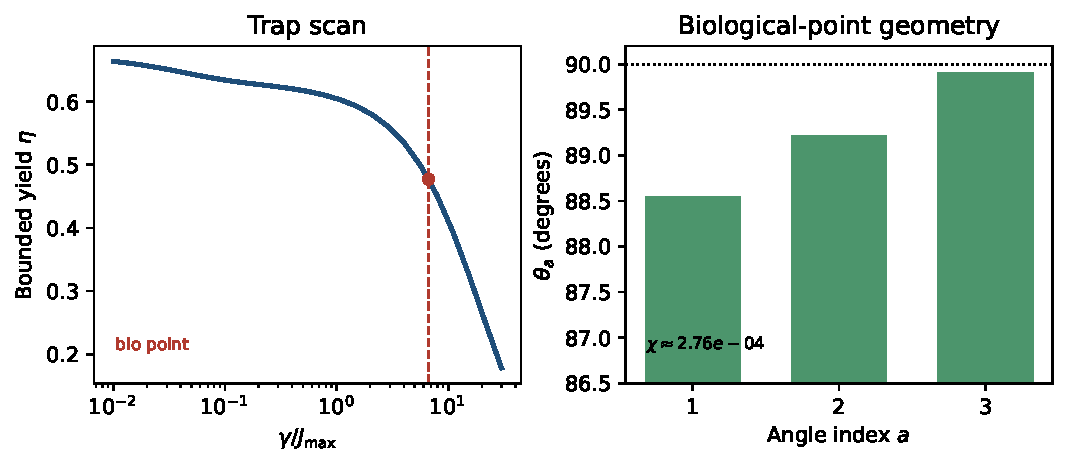
\includegraphics[width=0.92\linewidth]{ion_channel_anchor.pdf}
\caption{Ion-channel payload anchor. Left: $\theta_{\min}$ for the KcsA-like 4-site model as a function of $\gamma/J_{\max}$, with the biological point marked. Right: the three Bures principal angles at the biological point. At $\gamma_{\mathrm{bio}}/J_{\max}=6.67$, the ion-channel payload remains boundary-near with $\theta_{\min}\approx 88.55^\circ$ and $\chi\approx 2.76\times10^{-4}$.}
\label{fig:ion-channel-anchor}
\end{figure}

The role of the model is intentionally narrow: it establishes a concrete boundary-near payload anchor. If each channel carries only a very small local load, the aggregate payload can still be large whenever many channels are entrained and redundancy is not overwhelming.

A compact robustness sweep confirms this is not a one-point artifact. Varying $J_{\max}\in\{15,20,30,40\}$\,cm$^{-1}$ and $\gamma\in\{100,150,200,250,300\}$\,cm$^{-1}$ keeps $\theta_{\min}$ between $86.43^\circ$ and $88.93^\circ$ and $\chi$ between $1.53\times10^{-4}$ and $1.55\times10^{-3}$ across the entire $20$-point grid. A tighter topology sweep (varying inner-well asymmetry $\Delta\in\{10,15,20\}$\,cm$^{-1}$ and next-nearest coupling $J_2\in\{0,5,10\}$\,cm$^{-1}$ at fixed $J_{\max}=30$, $\gamma_{\mathrm{bio}}=200$\,cm$^{-1}$) keeps $\theta_{\min}$ between $88.55^\circ$ and $88.77^\circ$ and $\chi$ between $2.20\times10^{-4}$ and $2.77\times10^{-4}$. The anchor is parameter-sensitive but not a one-point artifact.

\subsection{Protein microdomains as secondary payloads}

Protein-folding microdomains, ligand-binding pockets, and other conformational substructures remain secondary in this paper. To represent that class explicitly, we use an illustrative coarse-grained $d=6$ mid-fold network,
\begin{equation}
H_{\mathrm{fold}}=
\begin{pmatrix}
20 & 25 & 12 & 0 & 0 & 0 \\
25 & 35 & 18 & 22 & 0 & 0 \\
12 & 18 & 42 & 20 & 10 & 0 \\
0 & 22 & 20 & 50 & 24 & 12 \\
0 & 0 & 10 & 24 & 38 & 26 \\
0 & 0 & 0 & 12 & 26 & 28
\end{pmatrix},
\end{equation}
with initial site $0$, target site $5$, $\kappa=0.5$\,ps$^{-1}$, and illustrative biological dephasing $\gamma_{\mathrm{bio}}=200$\,cm$^{-1}$. This is not a structure-specific folding Hamiltonian; it is a coarse molecular payload model intended to place a mid-fold microdomain in the same energy-scale analysis as the ion-channel anchor and the photosynthetic complexes \cite{dill2012protein}. The resulting values are $J_{\max}=26$\,cm$^{-1}$ and therefore $\gamma_{\mathrm{bio}}/J_{\max}\approx 7.69$. At the biological point the same Lindblad-plus-geometry pipeline gives $\theta_{\min}\approx 88.21^\circ$ and $\chi\approx 3.66\times10^{-4}$, with a local load $L_{\mathrm{fold}}\approx 1.10\times10^{-2}$. So the folding microdomain lands in the same near-boundary band as the ion-channel payload.

\section{Multi-Scale Architecture: Simulation and Coordination}
\label{sec:consequences}

\subsection{Classical carriers, non-classical payloads}

Neural oscillations at behavioral timescales are expected to be deep classical carriers. Two reduced carrier proxies confirm the direction of that limit. For a synthetic $d=10$ gamma microcircuit, $\theta_{\min}\approx 89.78^\circ$ with $\chi\approx 3.72\times10^{-6}$ by the reference point $\gamma/J_{\max}=50$. For a reduced Potjans--Diesmann cortical-column proxy ($d=8$; based on \cite{potjans2014cell}), $\theta_{\min}\approx 89.37^\circ$ with $\chi\approx 2.83\times10^{-5}$ at the same reference point. Even the less classical of the two carriers still sits roughly $10\times$ below the ion-channel payload anchor in $\chi$. This separation is the feature that makes the carrier useful: a deep-classical carrier can propagate, synchronize, and entrain without adding significant geometric mixing of its own.

\begin{figure}[H]
\centering
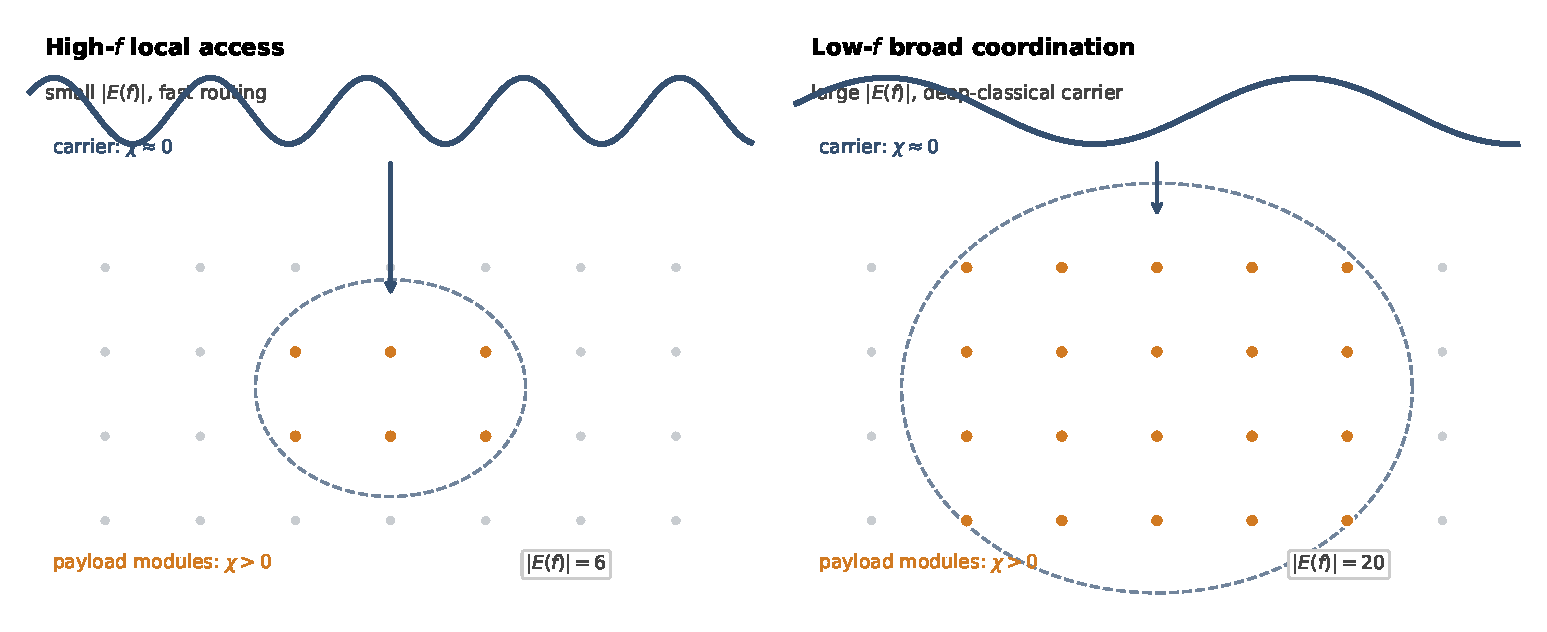
\includegraphics[width=0.92\linewidth]{carrier_payload_schematic.pdf}
\caption{Conceptual carrier-payload architecture. Left: a faster carrier coordinates a relatively small payload set. Right: a slower, more classical carrier coordinates a much larger set of slightly non-classical molecular payload modules. Dimensionality scales with the coordinated payload, not with the internal complexity of the carrier waveform.}
\label{fig:carrier-payload-schematic}
\end{figure}

One consequence of the carrier-payload split is that dimensionality in multi-scale biological systems need not live in carrier frequency. If lower-frequency carriers entrain larger cortical territories and therefore larger ion-channel payload sets \cite{buzsaki2012mechanisms}, then Corollary~\ref{cor:lowf} implies higher coordinated dimensionality even when the carrier is more classical. This reframes the intelligence question: one should look for the geometry of the coordinated substrate, not just the spectral properties of the carrier \cite{rigotti2013importance,fusi2016neurons}.

\subsection{Hybrid simulation protocol}
\label{sec:simulation}

The carrier-payload architecture implies a concrete simulation prescription for multi-scale biological systems. Classical simulation is appropriate whenever $\chi\approx 0$. For modules where $\chi > 0$, the non-classical payload is geometrically structured and should not be projected away without assessing the cost.

The resulting hybrid protocol has three layers:
\begin{enumerate}[label=(\roman*)]
\item \emph{Carrier layer.} Classical oscillatory dynamics (ODEs/PDEs for field propagation, phase coupling, amplitude envelope). This layer is already well handled by standard computational neuroscience tools and scales with conventional methods.
\item \emph{Payload layer.} Independent small open-quantum-system simulations. Each module of dimension $d$ requires a $d\times d$ Lindblad equation --- individually inexpensive. When inter-module quantum correlations are negligible, the number of independent simulations grows linearly with entrained territory rather than exponentially in composite Hilbert-space dimension.
\item \emph{Coupling layer.} The carrier determines which payload modules are entrained via phase-tolerant soft coupling (Section~\ref{sec:bridge}). Payload modules feed back to the carrier through population-level classical observables.
\end{enumerate}

The $\chi$ index serves as a screening heuristic: modules with $\chi$ well below the payload band ($\sim 10^{-4}$) are candidates for purely classical simulation, while modules in or above that band are flagged for Lindblad treatment. Whether a given $\chi$ threshold bounds surrogate error on observables of interest is itself an empirical question that the protocol is designed to answer.

A direct test of whether the non-classical payload matters computationally is to compare the hybrid simulation against a purely classical surrogate in which $\mathcal{L}_{\mathrm{eff}}$ is projected to zero (i.e., each module is replaced by its decohered classical populations). If the two simulations agree on all biologically measurable outputs --- dimensionality measures, synchronization patterns, information capacity --- then the payload is computationally inert and the framework's conjecture is falsified. If they diverge, even modestly, the payload contributes to the system's accessible dynamics in a way that classical simulation alone cannot capture.

This protocol is most practical for systems where the carrier dynamics are already well characterized (neural oscillations, circadian rhythms, developmental oscillators), the payload module class has a validated or estimable Hamiltonian (ion channel selectivity filters, photosynthetic reaction centers, enzyme active sites), and the readout is a classical observable that depends on the coordinated state of many modules.

\subsection{Soft phase-coupling carrier model}
\label{sec:bridge}

The remaining question is how carrier frequency enters the picture dynamically. Let a carrier of frequency $f$ propagate with speed $v$ and amplitude attenuation length $\lambda$. We assign each payload module a continuous coupling weight via an amplitude-decay kernel and a phase-compatibility kernel:
\begin{equation}
\label{eq:entrained-set}
w_A(r)=\exp\!\left[-\left(\frac{r}{R_{\mathrm{amp}}}\right)^\eta\right],
\qquad
w_\phi(r,f)=\exp\!\left[-\left(\frac{r}{R_\phi(f)}\right)^\eta\right],
\end{equation}
where $R_{\mathrm{amp}}=\lambda$ is the amplitude scale, $R_\phi(f)=v\Delta\phi_{\max}/(2\pi f)$ is the phase-limited coordination radius, and $\eta\ge1$ controls sharpness. Their product gives a combined weight
\begin{equation}
\label{eq:dcoord-scaling}
w(r,f)
=
\exp\!\left[-\left(\frac{r}{R_{\mathrm{eff}}^{(\eta)}(f)}\right)^\eta\right],
\qquad
R_{\mathrm{eff}}^{(\eta)}(f)=
\left(R_{\mathrm{amp}}^{-\eta}+R_\phi(f)^{-\eta}\right)^{-1/\eta}.
\end{equation}
If payload modules populate an effective spatial support of dimension $s$ with spatial density $\nu_m$, then the weighted payload size is
\begin{equation}
\label{eq:soft-payload-count}
\widetilde N(f)=
\nu_m C_s \Gamma\!\left(1+\frac{s}{\eta}\right)
\left(R_{\mathrm{eff}}^{(\eta)}(f)\right)^s,
\end{equation}
where $C_s=\pi^{s/2}/\Gamma(s/2+1)$ is the volume of the unit $s$-ball. In the phase-limited regime $R_\phi(f)\ll R_{\mathrm{amp}}$, $\widetilde N(f)\propto f^{-s}$; at sufficiently low frequency the growth saturates at the amplitude ceiling.

\begin{proposition}[Soft phase-coupling scaling with saturation]
\label{prop:threshold-scaling}
Assume the soft phase-coupling model above, a common payload dimension $d_m$, and the nonzero-density/bounded-redundancy conditions of Proposition~\ref{prop:extensive}. Then
\begin{equation}
D_{\mathrm{coord}}(E(f))
\ge
\nu_m C_s \Gamma\!\left(1+\frac{s}{\eta}\right)
\left(R_{\mathrm{eff}}^{(\eta)}(f)\right)^s
\left[(d_m-1)+\frac{pL_\star}{\varrho_\star}\right].
\end{equation}
In the phase-limited regime, coordinated dimensionality grows as $f^{-s}$; in the amplitude-limited regime, it saturates. The low-frequency advantage comes from coordinating a larger payload set, not from the carrier itself becoming less classical.
\end{proposition}

\begin{proof}
Equation~\eqref{eq:soft-payload-count} gives the weighted payload size. For modules of common dimension $d_m$, Definition~\ref{def:payload} gives $D_{\mathrm{coord}}(E(f))=\widetilde N(f)(d_m-1)+\mathcal{L}_{\mathrm{eff}}(E(f))$. Applying Proposition~\ref{prop:extensive} to the weighted entrained set yields $\mathcal{L}_{\mathrm{eff}}(E(f))\ge (pL_\star/\varrho_\star)\widetilde N(f)$, which gives the stated bound.
\end{proof}

Proposition~\ref{prop:threshold-scaling} is a toy bridge. It does not fit real cortical attenuation, conduction anisotropy, or laminar structure. Its role is to make the paper's inversion explicit in a model with continuous coupling, finite propagation, and smooth saturation.

Figure~\ref{fig:threshold-scaling} overlays a heterogeneous soft-field simulation to check that the low-frequency advantage is not an artifact of a hard threshold. With $12{,}000$ payload modules across a 2D disc, lognormally distributed amplitude and phase scales, and normalization at $f=f_0$, the resulting payload load remains monotone as frequency falls and gives approximately $3\times$ gain at beta frequencies ($20$\,Hz, taking $f_0=40$\,Hz as gamma reference), $\sim\!10\times$ at theta ($6$\,Hz), with smooth saturation through delta and infraslow. A coarse sensitivity sweep across $s\in\{1,2,3\}$, $\eta\in\{1,2,4\}$, and $R_{\mathrm{amp}}/R_0\in\{2,4,8\}$ keeps the gain monotone in all cases.

Using the ion-channel anchor, the local non-classical load is
\begin{equation}
\label{eq:lion}
L_{\mathrm{ion}}=\chi(d^2-d)\approx (2.76\times 10^{-4})\times 12 \approx 3.31\times 10^{-3}
\end{equation}
per channel. For homogeneous payload modules, the fractional uplift above the classical baseline is
\begin{equation}
\label{eq:uplift-fraction}
\Phi = \frac{\chi d_m}{\varrho}.
\end{equation}
For the ion-channel anchor ($d_m=4$),\ $\Phi_{\mathrm{ion}}\approx 1.10\times10^{-3}/\varrho$. The per-channel effect is small, but the absolute payload is extensive in $N$. Whether this fractional uplift is functionally amplified by real biological dynamics is an empirical question --- precisely the question the simulation protocol in Section~\ref{sec:simulation} is designed to answer.

\begin{figure}[H]
\centering
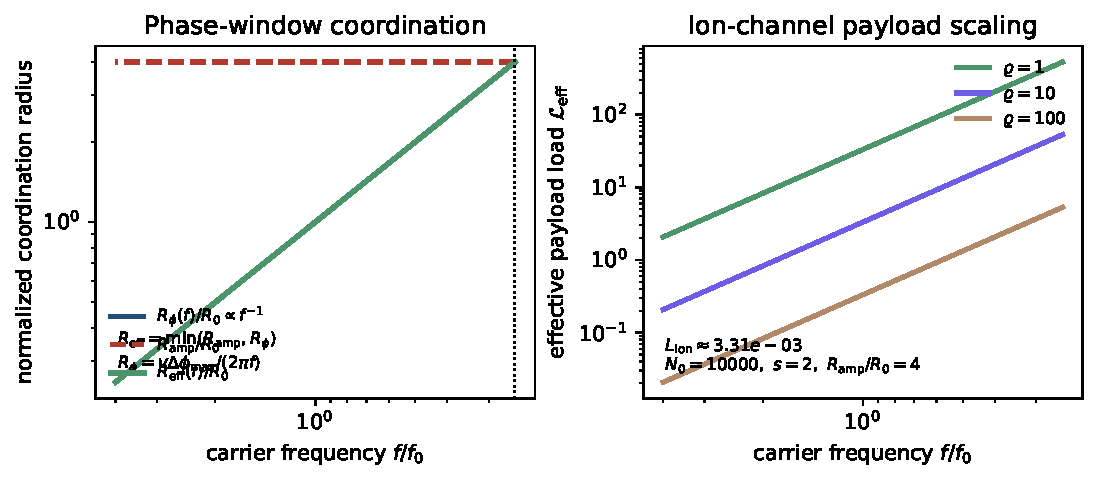
\includegraphics[width=0.92\linewidth]{threshold_entrainment_scaling.pdf}
\caption{Soft phase-coupling bridge. Left: the phase-limited radius $R_{\phi}(f)$ and amplitude scale $R_{\mathrm{amp}}$ combine into a soft-min radius $R_{\mathrm{eff}}^{(\eta)}(f)$. Right: dashed curves show the analytic soft payload load for illustrative $N_0=10^4$, $s=2$, $R_{\mathrm{amp}}/R_0=4$, $\eta=2$, and redundancy factors $\varrho\in\{1,10,100\}$. Solid curves show a heterogeneous soft-field simulation with distributed amplitude and phase tolerances. The low-frequency advantage and smooth saturation survive heterogeneity.}
\label{fig:threshold-scaling}
\end{figure}

\subsection{Empirical predictions}

The carrier-payload framework yields predictions that distinguish it from a purely frequency-driven account of neural dimensionality. Table~\ref{tab:rival-predictions} states the contrast in operational form.

\begin{table}[H]
\centering
\small
\begin{tabularx}{\linewidth}{@{}>{\raggedright\arraybackslash}p{3.2cm}YY@{}}
\toprule
Observable or manipulation & Frequency-dominant expectation & Carrier-payload expectation \\
\midrule
Cross-condition variation in measured dimensionality & Dimensionality should increase primarily with carrier frequency or burstiness. & Dimensionality should increase primarily with entrained payload size and payload diversity, even when the carrier is slower. \\
Hold carrier coherence fixed while reducing available payload sites & Only modest changes if the carrier spectrum is preserved. & Effective dimensionality should fall because the payload is where state-space richness resides. \\
Compare low-frequency broad-coordination states with high-frequency local-access states & High-frequency states should appear more dimensional. & Low-frequency states can appear more dimensional when they coordinate a larger payload ensemble. \\
\bottomrule
\end{tabularx}
\caption{Alternative empirical expectations. The paper does not deny that high-frequency bursts can correlate with flexible access or gating \cite{lundqvist2016gamma,miller2018working}. It denies the stronger inference that carrier frequency itself is the primary locus of dimensionality.}
\label{tab:rival-predictions}
\end{table}

The framework is testable without direct molecular-state tomography. Table~\ref{tab:measurement-program} maps the theoretical objects onto experimental proxies.

\begin{table}[H]
\centering
\small
\begin{tabularx}{\linewidth}{@{}>{\raggedright\arraybackslash}p{3.05cm}YY@{}}
\toprule
Theoretical object & Practical proxy & Carrier-payload expectation \\
\midrule
Carrier coherence & Low-frequency phase locking, coherence radius, or cross-area synchrony & A more reliable carrier should enlarge entrained territory, not increase dimensionality through frequency alone. \\
Entrained payload size $\lvert E(f)\rvert$ & Spatial footprint of phase-locked tissue or effective coordination territory & Larger coordinated territory should predict larger measured dimensionality, conditional on comparable payload statistics. \\
Payload diversity & Channel/receptor diversity, pharmacological conductance availability, or cell-type conductance richness & Reducing payload diversity at fixed carrier coherence should reduce dimensionality. \\
Observed dimensionality & Participation ratio, manifold dimension, shattering dimension, or mixed-selectivity capacity \cite{rigotti2013importance,fusi2016neurons} & Dimensionality should be better explained by coordinated territory and payload diversity than by carrier frequency alone. \\
\bottomrule
\end{tabularx}
\caption{Operational measurement route. The proposal requires testing whether recorded dimensionality is better predicted by coordinated territory and payload diversity than by carrier frequency alone.}
\label{tab:measurement-program}
\end{table}

A minimal empirical test at the level of recorded neural data:
\begin{equation}
\label{eq:empirical-test}
D_{\mathrm{obs}}
=
\beta_0
+\beta_1 \log \widetilde N
+\beta_2 H_{\mathrm{payload}}
+\beta_3 C_{\mathrm{carrier}}
+\beta_4 \log f
+\varepsilon,
\end{equation}
where $D_{\mathrm{obs}}$ is an observed dimensionality measure, $\widetilde N$ is coordinated territory, $H_{\mathrm{payload}}$ is a payload-diversity proxy, and $C_{\mathrm{carrier}}$ is a carrier-coherence proxy. The carrier-payload picture predicts $\beta_1,\beta_2>0$ and that $\beta_4$ should shrink toward zero once the other controls are included. The frequency-dominant interpretation predicts the opposite.

\section{Discussion}
\label{sec:discussion}

The main contribution of this paper is a geometric framework for understanding where biological systems sit on the quantum-classical boundary and what follows from that position. Decoherence is a dimensional projection of state space. The $\chi$ index turns that projection into a continuous, computable measure. Applied to biology, it reveals a consistent pattern: molecular payload modules (photosynthetic complexes, ion channel selectivity filters, protein microdomains) inhabit a near-boundary band with small but nonzero $\chi$, while macroscopic carrier dynamics are already deep classical. This carrier-payload separation is the paper's central model-based observation.

\subsection{Connection to Igamberdiev's program}

Igamberdiev and colleagues have long argued that biological systems operate productively at the quantum-classical border and that this boundary position is not incidental but functionally exploited \cite{igamberdiev1993,igamberdiev2021qcborder}. The present framework provides a geometric formalization of that insight. The $\chi$ index is, in effect, a coordinate on Igamberdiev's border: it says not just that a system is near the boundary, but \emph{how near}, in which geometric directions, and with what aggregate load across a multi-module assembly. The extensive-payload result (Proposition~\ref{prop:extensive}) gives formal content to the idea that biological complexity can accumulate non-classical resources: if a nonzero fraction of molecular modules sits near the boundary, the total payload scales with system size rather than saturating.

The carrier-payload architecture also connects to the broader theme of multi-scale temporal organization in living systems \cite{igamberdiev2014}. Classical carriers provide the temporal scaffolding --- the oscillatory coordination that biology uses to organize activity across spatial and temporal scales. The payload is where the fine-grained state-space structure resides. This is a division of labor: the carrier handles synchronization (a classical strength), while the payload retains geometric richness (a near-boundary property).

\subsection{Simulation implications}

The hybrid simulation protocol in Section~\ref{sec:simulation} is perhaps the most immediately practical consequence of the framework. Current practice in computational biology faces a dilemma: full quantum simulation of biological systems is exponentially expensive, while purely classical simulation projects away whatever non-classical payload the system carries. The carrier-payload framework resolves this by providing a principled classification criterion. Modules with $\chi\approx 0$ need only classical treatment. Modules with $\chi > 0$ require small open-quantum-system simulations that are individually cheap and collectively scale linearly.

The critical empirical test is whether the hybrid and classical-only simulations diverge on biologically measurable outputs. If they do not, the non-classical payload is computationally inert and the framework's conjecture is falsified. If they do --- even at the modest fractional uplift $\Phi_{\mathrm{ion}} \approx 10^{-3}/\varrho$ implied by the ion-channel anchor --- the divergence identifies exactly which aspects of biological dynamics require quantum treatment and which do not. Either outcome is informative.

\subsection{A speculative engineering direction}

The carrier-payload architecture also suggests a hypothesis about engineered computing systems. Standard quantum computing isolates qubits from their environment to maintain coherence, paying enormous overhead in error correction and cryogenic cooling. The present framework points toward a different question: could one accept partial decoherence at the module level, use a classical oscillatory backbone for synchronization and routing, and compensate with horizontal scaling --- many slightly non-classical processing elements coordinated by a deep-classical carrier? In such an architecture the computational resource would not be qubit fidelity but coordinated payload breadth.

Whether this architecture can achieve advantages over purely classical systems of the same physical size depends on whether the geometrically accessible coherence directions opened by the payload enable state-space exploration that classical trajectories cannot replicate. The biological existence proof --- billions of years of evolution producing carrier-payload architectures at ambient temperature --- suggests the question is worth posing concretely. It also suggests that the right engineering target is not maximal coherence but optimal boundary position: the $\chi$ that maximizes useful payload at the available thermal and coupling scales.

\subsection{Limitations and open questions}

Several things remain open. The current analysis includes reduced photosynthetic anchors, two neural payload anchors, and two carrier proxies, but does not span the broader family of molecular payload models. The redundancy factor $\varrho_E$ needs empirical grounding. The soft phase-coupling bridge is explicitly a toy model. And the simulation protocol has not yet been implemented on a data-constrained biological system. These are real gaps. They are also the right gaps: they are downstream of a coherent framework rather than upstream of one.

The paper does not claim that neural oscillations are quantum, that high dimensionality forces non-classicality, or that the non-classical payload is already known to be functionally decisive. It claims that biological systems built from many structured molecular machines can carry an extensive non-classical payload if a nonzero density of those machines sits near the quantum-classical boundary; that the carrier-payload architecture provides a principled simulation framework; and that the whole picture is directly testable. The numerical lesson is sober: the local fractional uplift is small [Eq.~\eqref{eq:uplift-fraction}], but the absolute payload remains extensive in entrained site count, and whether that matters functionally is an empirical question that the framework is designed to resolve.

\section*{Data and Code Availability}

All code used to generate the results and figures in this manuscript is available at:
\href{https://github.com/todd866/decoherence-dimensional-collapse}{github.com/todd866/decoherence-dimensional-collapse}.

\section*{Funding}

No specific external funding supported this work.

\section*{CRediT Authorship Contribution Statement}

Ian Todd: Conceptualization, Methodology, Software, Formal analysis, Visualization, Writing---original draft, Writing---review \& editing.

\section*{AI Use Disclosure}

AI-assisted tools were used for code generation, numerical workflow iteration, and editorial revision. All mathematical claims, model choices, code paths, figures, and manuscript statements were checked and curated by the author.

\bibliographystyle{unsrt}
\bibliography{references}

\end{document}
